\documentclass[a4paper,ngerman]{article}

\usepackage{babel}
\usepackage[utf8]{inputenc} 
\usepackage[T1]{fontenc} 
\usepackage{tabularx}
\usepackage{graphicx}
\usepackage{listings}

\author{Paul Podlech \\ 3910583 \and Max Wisniewski\\4370074}
\title{Mikroprozessor Praktikum\\ Fr. HWP 2 \\ Aufgabenblock 1}
\date{\today}

\begin{document}

\lstset{language=C, basicstyle=\ttfamily\fontsize{10pt}{10pt}\selectfont\upshape, commentstyle=\rmfamily\slshape, keywordstyle=\rmfamily\bfseries, breaklines=true, frame=single, xleftmargin=3mm, xrightmargin=3mm, tabsize=2, mathescape=true, numbers=left}

\maketitle

\newpage

\section*{Aufgabe 1: I/O Pots}

\subsection*{Output}

\begin{description}

\item{\bfseries A1.1.1}

Klären Sie die Funktion folgender Register:

\begin{description}

\item{\bfseries P4Sel:} Mit diesem Register kann man das Signal von oder an ein internes Modul weiterleiten. Das sorgt dafür, dass man entweder Daten direkt verarbeiten kann ohne das die CPU mitarbeiten muss, oder Signale automatisch rausgeschickt werden können, wie eine Lampe die im Takt blinken soll. Dabei steht \textbf{0} für I/O Funktionalität und \textbf{1} für Modul Funktionalität.

\item{\bfseries P4Dir:}  Legt fest, ob man von diesem Port liest oder auf ihn raus schreiben möchte. Dabei steht:\\
\textbf{0} für \emph{IN}, das heißt man will lesen und\\
\textbf{1} für \emph{OUT}, das heißt man will schreiben. 

\item{\bfseries P4Out:} Hier schreibt man die Daten hinein, wenn man etwas senden möchte. Sobald Direction auf \emph{OUT} steht, ist dieses Signal aussehn sichtbar.


\item{\bfseries P4In:} Von hier kann gelesen werden, welches Signal am vierten Port anliegt, wenn die Direction am \emph{P4Dir} auf \emph{IN} steht. Allerdings reflektiert es auch im \emph{OUT} Fall den Wert, den wir selber setzen.

\end{description}

Dies ist für für alle Ports gleich, wobei man für die anderen Ports die 4 durch die entsprechende Portnummer ersetzen muss.

\item{\bfseries A 1.1.2}

Erstellen Sie eine Liste von Bitoperationen auf und geben Sie Operationen zum Setzen, Toggeln, Rücksetzen an.

\begin{tabular}{c|c|c}

Name & Beschreibung & Symbol\\
\hline

AND & Verunded die die Zahlen Bitweise &  \&\\

OR & Verodert die Zahlen Bitweise & | \\

XOR &  VerXORt die zaheln Bitweise & HOCH \\

Komplement &  Bildet das Bitweise Komplemet & \textasciitilde \\

Rechtshift & Shiftet die Bits nach rechts und füllt mit 0en & >>\\

Linksshift & Shiftet die Bits nach links und füllt mit 0en & <<\\

\end{tabular}

\begin{description}

\item{\bfseries Setzen:} $P4OUT \; |= 1<< k$. Setzt das k-te Bit auf 1. Um mehrere Bits zu setzen, können wir mit der Bitmaske verodern, die an allen Stellen eine 1 hat, die wir setzen wollen und eine 0 sonst.

\item{\bfseries Toggeln:} $P4OUT \;  XOR= 1<<k$ Setzt das k-te Bit auf sein Komplement. Um mehrere Bits zu setzen, können wir mit der Bitmaske verodern, die an allen Stellen, die wir Toggeln wollen eine 1 und sonst eine 0.

\item{\bfseries Zurücksetzen:} $P4OUT \; \&= \textasciitilde (1<<k)$. Die Bitmaske hat an der k-ten Stelle eine 0 und sonst 1en. Damit Wird die k-te Stelle auf 0 gesetzt. Um mehrere Bits zu setzen, können wir mit der Bitmaske verunden, die an jeder Stelle eine 0 hat, die wir zurück setzen wollen und sonst 1en.

\end{description}

\item{\bfseries A1.1.3} Erläutern Sie anhand der Abbildung der internen Struktur einer Portleitung für die folgende Registerbelegung den Signalpfad und den Logikpegel der Portleitung P4.0

\begin{itemize}
\item define LED\_ROT(0x01)
\item P4SEL = 0x00
\item P4DIR = 0x0F
\item P4OUT |= LED\_ROT

\end{itemize}

Daraus könen wir herraus lesen, dass Select für alle auf 0 steht, dass heißt es ist als I/O Port geschaltet. Die Direction von 0x0F heißt, dass für Bit 0 eine 1 anliegt (da die unteren 4 Bit gesetzt sind). Wenn LED\_ROT mit unserem OUT verodert wird, kann man, wie in der letzen Aufgabe gezeigt, heißt dass, dass das 0te Bit gesetzt wird.\\

\begin{figure}[h!]
	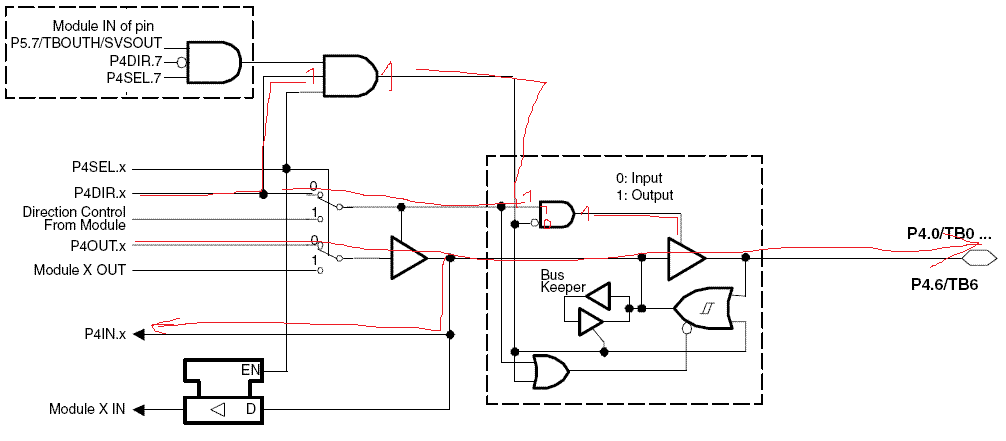
\includegraphics[scale=0.6]{1_3.png}
\end{figure}

Aus unserem Bild kann man herrauslesen, das an P4.0 eine 1 herraus kommt.

\item{\bfseries A 1.1..4} Die LED leuchted, wenn wir eine Potentialdifferenz über der LED haben. Da auf der rechten Seite der LED eine Betriebsspannung (von 3V) anliegt, wie man aus dem Schaltbild lesen kann, benötigen wir ein niedrigeres Potential, damit ein Strom fließen kann. Diese wird bei 0 erreicht, da die Spannung zwischen den beiden Potentialen dann groß genug ist. Bei einem Highpegel wird diese Differenz 0 sein.

\pagebreak

\item{\bfseries A 1.1.5} Erläutern Sie inhaltlich die Bedeutung der folgenden Codezeilen:

\begin{lstlisting}
unsigned char a;
#define LEDRT (0x01)
P4DIR = 0x00;
a = 10;
P4OUT = a;
P4OUT = 0x01;
P4DIR = 0x07;
P4OUT = 0x00;
P4OUT |= 0x01;
P4OUT |= LEDRT;
P4OUT ^= ~LEDRT;
P4OUT ^= LEDRT;
\end{lstlisting}

Direction wird 2 mal gesetzt. Nach der ersten Anweisung wird alles auf eingang gesetzt und außen ist nichts zusehen. Nach der zweiten können wir an Leitung P4.0, P4.1, P4.2 ein Signal sehen.\\
Die Zeilen 5,6 haben keine Auswirkungen, da sie nicht sichtbar sind nach außen.\\
Nach Zeile 7 können wir die 1 auf P4.0 sehen, die in 6 gesetzt wurde.\\
Nach Zeile 8 können wir von außen an P4.0, P4.1, P4.2 eine 0 sehen.\\
Nach Zeile9 wurde auf P4.0 eine 1 gesetzt.\\
Nach Zeile 10 hat sich nichts geändert, da das Bit 0 schon vorher gesetzt wurde.\\
Nach Zeile 11 wurde mit dem komplement von LEDRT getoggelt. Das heißt, dass P4OUT nun 0xFF ist. Jedes Bit ist 1 und damit ist an P4.0, P4.1, P4.2 diese auch zu sehen. Die anderen Bits sind immer noch nicht auf OUT geschaltet.\\
Nach Zeile 12 wurde Bit 0 wieder getoggelt. Das bedeutet das an P4.0 eine 0 anliegt und an P4.1, P4.2  weiter die 1 bleibt.

\pagebreak

\item{\bfseries A 1.1.6} Schreiben Sie ein Programm, dass die Phasen ein Ampel durchläuft. Und zwischen den einzelnen Phasen immer etwas Zeit lässt.\\
Wir haben uns dafür Makros für die Werte von Rot, Gelb und Grün geschrieben. Diese werden immer Program immer wieder kombiniert und dan auf die Outleitung gesetzt. Beim Aufruf haben wir als erstes darauf geachtet, dass die Leitungs Direction erst auf OUT gesetzt wird, wenn wir im OUT was etwas reingeschrieben haben.

\begin{lstlisting}
#define	ROT		(0x01) // Bitmaske fuer rote LED
#define	GELB		(0x02) // Bitmaske fuer gelbe LED
#define	GRUEN	(0x04) // Bitmaske fuer gruene LED

void aufgabe1(){
	P4SEL		=	0x00;	 // setze den gesammten Port auf OUT
	P4DIR		=	7	 // setzt LED Leitungen auf OUT
	P4OUT	=	~ROT; //setzt die rote LED
	wait(50000);
	wait(50000);
	P4OUT	=	~( ROT | GELB); //setzt sowohl die rote als auch die gelbe LED
	wait(50000);
	P4OUT	= 	~(GRUEN);	 //setzt die gruene LED
	wait(50000);
	wait(50000);
	P4OUT	=	~(GELB)	 // gelbe LED auf an
	wait(50000);
}
\end{lstlisting}

Wir haben uns an dieser Stelle für die einfache Lösung entschieden und überschreiben alle Bits, die wir nicht setzten wollen. Dies könnte man umgehen indem man die Bits an sich setzt. Da in unserem Programm aber nicht mehr passiert, ist das an dieser Stelle vertretbar.

Unsere Beobachtungen waren: Es funktioniert.

\end{description}

\end{document}